\newcommand\N{\ensuremath{\mathbb{N}}} 
\newcommand\R{\ensuremath{\mathbb{R}}} 
\newcommand\A{\ensuremath{\mathbb{A}}} %affine space
\newcommand\Z{\ensuremath{\mathbb{Z}}} 
\renewcommand\O{\ensuremath{\emptyset}} 
\newcommand\Q{\ensuremath{\mathbb{Q}}} 
\newcommand\C{\ensuremath{\mathbb{C}}}
\newcommand\F{\ensuremath{\mathbb{F}}} %field
\newcommand\E{\ensuremath{\mathbb{E}}} %field extension
\renewcommand\P{\ensuremath{\mathbb{P}}} %projective space
\renewcommand\H{\ensuremath{\mathbb{H}}} %hyperbolic space
\newcommand\im{\ensuremath{\operatorname{im}}} %image
\newcommand\rank{\ensuremath{\operatorname{rank}}} %rank
\newcommand\id{\ensuremath{\operatorname{id}}} %identity map
\newcommand\grad{\ensuremath{\operatorname{grad}}} %gradient
\newcommand\curl{\ensuremath{\operatorname{curl}}} %gurl
\renewcommand\div{\ensuremath{\operatorname{div}}} %divergence
\newcommand\Gr{\ensuremath{\operatorname{Gr}}} %grassmannian
\newcommand\Hom{\ensuremath{\operatorname{Hom}}} %linear mappings

\documentclass[xcolor=dvipsnames]{beamer} 
\usetheme{Copenhagen} 
\beamertemplatenavigationsymbolsempty
\definecolor{burntorange}{RGB}{191,87,0}
\definecolor{utgrey}{RGB}{51,63,72} 

\setbeamercolor{palette primary}{bg=burntorange,fg=white}
\setbeamercolor{palette secondary}{bg=burntorange,fg=white}
\setbeamercolor{palette tertiary}{bg=burntorange,fg=white}
\setbeamercolor{palette quaternary}{bg=burntorange,fg=white}
\setbeamercolor{structure}{fg=burntorange} % itemize, enumerate, etc
\setbeamercolor{section in toc}{fg=burntorange} % TOC sections
\setbeamercolor{subsection in head/foot}{bg=burntorange,fg=white}
\setbeamercolor{block title example}{fg=white,bg=burntorange}
%\setbeamercolor{block body example}{fg=white,bg=burntorange}

\usepackage[utf8]{inputenc} 
\usepackage{float}
\usepackage{tikz} 
\usepackage{tikz-cd} 
\renewcommand\qedsymbol{$\boxtimes$}
\title{An introduction to de Rham cohomology} 
\subtitle{How algebra and calculus relate to topology} 
\author{Simon Xiang} 
\institute{University of Texas at Austin} 
\begin{document} 
    \begin{frame}
        \titlepage
    \end{frame}

    %\begin{frame}
        %\frametitle{Prerequisites} 
        %Here are some things I'll assume you know about:
        %\begin{itemize}
            %\item Linear algebra, including quotient spaces, exact sequences,
            %\item Basic multivariable calculus,
            %\item What an open set is,
        %\end{itemize}
        %It would be helpful to know 
        %\begin{itemize}
            %\item Basic algebraic structures, notably groups and algebras,
            %\item And some topology.
        %\end{itemize}
    %\end{frame}

    \begin{frame}
        \frametitle{Motivation} 
        \begin{exampleblock}{Question} 
            Does there exist a function that is the gradient of some other function? More precisely, when does there exists an $F \colon U \to \R^2$ for some open $U \subseteq \R^2$ that satisfies \[
                \frac{\partial F}{\partial x}=f_1,\quad \frac{\partial F}{\partial y}=f_2 \quad \text{for a vector field} \ f=(f_1,f_2)?
            \] (You could also think of this question as asking when vector fields have potential.)
        \end{exampleblock}\pause
        \begin{exampleblock}{Answer} 
           It depends on the topology of $U$! 
        \end{exampleblock}
    \end{frame}
    

    \begin{frame}
    \frametitle{Some vector calculus} 
    Note that $\frac{\partial F}{\partial x}=f_1,\ \frac{\partial F}{\partial y}=f_2$ implies $\frac{\partial f_1}{\partial y}=\frac{\partial f_2}{\partial x}$. Is this condition sufficient to show $F$ is the gradient of some other function?
    \begin{example}
        The vector field $f(x,y)=(y,x)$ satisfies $\frac{\partial f_1}{\partial y}= \frac{\partial f_2}{\partial x}=1$, and the gradient of $F=xy$ is $f$.
    \end{example}%\pause
    \begin{example}
        \begin{columns}
            \column{0.5\textwidth} 
            However, consider $f(x,y)=\left( \frac{-y}{x^2+y^2},\frac{x}{x^2+y^2} \right) $. This vector field cannot be conservative, which you can show by integrating around a closed loop.
            \column{0.3\textwidth} 
            \begin{figure}[H]
            \centering
             \includegraphics[width=1\linewidth]{derham1.png}
            \end{figure}
        \end{columns} 
    \end{example}
    \end{frame}
    \begin{frame}
    \frametitle{Div, grad, curl} 
    \begin{block}{Proposition} 
                \begin{columns}
            \column{0.7\textwidth} 
        The condition $\frac{\partial f_1}{\partial y}=\frac{\partial f_2}{\partial x}$ is sufficient for the existence of a conservative vector field $F$ if $U$ looks like a ball (convex). 
            \column{0.2\textwidth} 
            \begin{figure}[H]
            \centering
             \includegraphics[width=0.6\linewidth]{convex.png}
            \end{figure}
        \end{columns} 

        %Note that $\R^2\setminus \{0\} $ is \emph{not} convex since you can't connect the points $(-1,0),(1,0)$ by a line.
    \end{block}
        %\begin{definition}
        %If $C^{\infty}(U,\R^k)$ denotes the set of smooth functions $U \to \R^k$ define the maps $C^{\infty}(U,\R) \overset{\grad}{\to } C^{\infty}(U,\R^2) \overset{\curl}{\to } C^{\infty}(U,\R),$ where $\operatorname{grad}(\phi)=\left( \frac{\partial  \phi}{\partial x}, \frac{\partial \phi}{\partial y} \right) ,\ \operatorname{curl}(\phi_1,\phi_2)=\frac{\partial \phi_1}{\partial y}-\frac{\partial \phi_2}{\partial x} $.
        %\end{definition}%\pause
        \begin{definition}
            Define $C^{\infty}(U,\R) \overset{\grad}{\to } C^{\infty}(U,\R^3)\overset{\curl}{\to } C^{\infty}(U,\R^3)\overset{\div}{\to } C^{\infty}(U,\R)$, 
        \begin{align*}
   \grad \colon &f \mapsto \left( \frac{\partial f}{\partial x},\frac{\partial f}{\partial y},\frac{\partial f}{\partial z} \right), \\
   \curl \colon   &(f_1,f_2,f_3) \mapsto \left( \frac{\partial f_3}{\partial y}-\frac{\partial f_2}{\partial z},\frac{\partial f_1}{\partial z}-\frac{\partial f_3}{\partial x},\frac{\partial f_2}{\partial x}-\frac{\partial f_1}{\partial y}\right), \\
\operatorname{div} \colon &(f_1,f_2,f_3) \mapsto \frac{\partial f_1}{\partial x}+\frac{\partial f_2}{\partial y}+\frac{\partial f_3}{\partial z}.
\end{align*}
        \end{definition}%\pause
    \end{frame}

    \begin{frame}
        \frametitle{Sneak peek of de Rham cohomology} 
        \begin{block}{Proposition} 
           The curl of the gradient is zero, or $\operatorname{curl}\circ \operatorname{grad}=0$. 
        \end{block}\pause
        This implies that $\operatorname{im}(\operatorname{grad}) \subseteq \ker (\operatorname{curl})$, so we can form the \emph{quotient space} $H^1(U):= \ker (\operatorname{curl})/ \operatorname{im}(\operatorname{grad})$. 
       \begin{definition}
            The space $H^1(U)$ is the \textbf{1st de Rham cohomology group} of $U$.        
        \end{definition}
        Now the aforementioned proposition is equivalent to saying $H^1(U)=0$ whenever $U$ is convex. Here's why:
        \begin{itemize}
            \item<2->All we need to show is that $\ker(\curl) \subseteq \im(\grad).$
            \item<3->In two dimensions, $f \in \ker(\curl)$ means $ \frac{\partial f_2}{ \partial x}-\frac{\partial f_1}{\partial y}=0$.
            \item<4->So $\frac{\partial f_1}{\partial y}= \frac{\partial f_2}{\partial x}$, and we know what to do from here!
        \end{itemize}
    \end{frame}

    \begin{frame}
    \frametitle{More on de Rham cohomology} 
\begin{block}{Proposition} 
$\div \circ \curl =0$.    
\end{block}
    \begin{definition}
    Since the composition $\div \circ \curl$ is zero, we can also form the \textbf{2nd de Rham cohomology group} $H^2(U):=\ker (\div) / \im(\curl)$. To fit with the theme, define $H^0(U)=\ker (\grad)$. 
    \end{definition}%\pause
    It turns out de Rham cohomology measures the amount of ``holes'' in a space. Since $\R^3$ is ``completely solid'', there should be no nontrivial de Rham cohomology. The following theorem demonstrates this.
   % Intuitively, $H^1(\R^2 \setminus \{0\} )\neq 0$ since this space has a nontrivial topology. But how do we show this?
    \end{frame}
    \begin{frame}[fragile]
        \frametitle{A quick summary} 
    \begin{theorem}
        For a convex open set $U \subseteq \R^3$, we have $H^0(U)=\R,\,H^1(U)=0,$ and $H^2(U)=0$.
    \end{theorem}\pause
    \begin{figure}[H]
    \centering
     \includegraphics[width=0.6\linewidth]{homotopy_circ.jpg}
    \end{figure}\pause
        %The relationships between divergence, gradient, and curl, and the 0th, 1st, and 2nd de Rham cohomology groups of a convex open subset of $\R^3$ can be summarized in the following commutative diagram:
        \begin{figure}[H]
    Note: This is not an actual commutative diagram!
        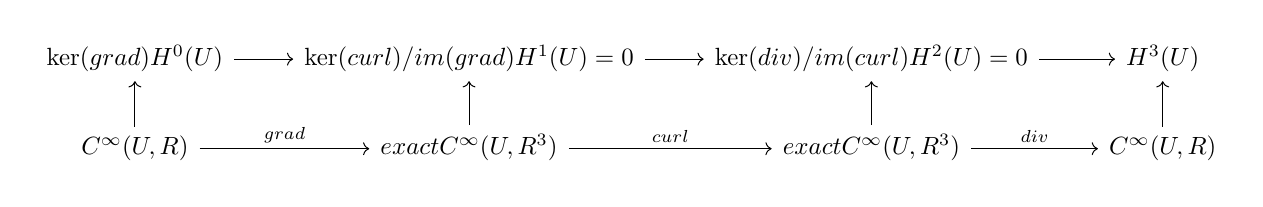
\begin{tikzpicture}[baseline= (a).base]
\node[scale=.9] (a) at (0,0){
        \begin{tikzcd}
        \overset{\ker(\grad)}{H^0(U)} \arrow[r]                       & \overset{\ker(\operatorname{curl})/\operatorname{im}(\operatorname{grad})}{H^1(U)=0 } \arrow[r] & \overset{\ker(\div)/\im(\curl)}{H^2(U)=0 } \arrow[r]                       & H^3(U)                       \\
        {C^{\infty}(U,\R)} \arrow[r, "\operatorname{grad}"] \arrow[u] & {\underset{\text{exact}}{C^{\infty}(U,\R^3)}} \arrow[r, "\operatorname{curl}"] \arrow[u]       & {\underset{\text{exact}}{C^{\infty}(U,\R^3)}} \arrow[u] \arrow[r, "\div"] & {C^{\infty}(U,\R)} \arrow[u]
        \end{tikzcd}
};
\end{tikzpicture}
        \end{figure}
    \end{frame}


    \begin{frame}
        \frametitle{The de Rham complex} 
        Let's shift gears to a more abstract setting.
        \begin{definition}
            Define $\Omega^*$ to be the algebra generated by $dx_1,\cdots ,dx_n $ with the relations \[
            \begin{cases}
                (dx_i )^2=0,\\
                dx_i dx_j =-dx_j dx_i ,\ i\neq j.
            \end{cases}
        \] Then a \textbf{differential form} is an element of $\Omega^*(U)$, formally defined as $C^{\infty}(U,\R)\otimes _{\R}\Omega^*$, where $U \subseteq \R^n $ is open. This algebra has a natural grading $\Omega^*(U)=\bigoplus _{q=0}^n \Omega^q(U)$.
        \end{definition}%\pause
    \begin{example}
        Concretely, a form $\omega \in  \Omega^q(U)$ can be written uniquely as $\sum f_I dx_I$, where $I$ denotes a strictly increasing sequence of length $q<n$.
    \end{example}
    \end{frame}

    \begin{frame}
        \frametitle{The exterior derivative} 
        \begin{definition}[]
            Define a \emph{differential operator} $d \colon \Omega^q(U) \to \Omega^{q+1} (U)$ by the following properties:
            \begin{enumerate}[i]
            \setlength\itemsep{0.2em}
        \item if $f \in \Omega^0(U)$, then $df=\sum \frac{\partial f}{\partial x^i }dx^i $,
        \item if $\omega =\sum f_I dx_I,$ then $d\omega=\sum df_Idx_I$.
            \end{enumerate}
            This operator is called \textbf{exterior differentiation.} 
        \end{definition}
        \begin{definition}[]
            The algebra $\Omega^*\left(U \right)$ paired with the differential operator $d$ is called the \textbf{de Rham complex} on $U$.
        \end{definition}%\pause
\begin{example}
    %A return to grounded reality. 
    Let $\omega=xy\,dx \in \Omega^1(\R)$ be a 1-form. Then $d \omega = \left( \frac{\partial (xy)}{\partial x}dx+ \frac{\partial (xy)}{\partial y}dy \right) dx=y\,dx\,dx+x \,dy\,dx=-x\,dx\,dy.$ We will see more exterior derivative calculations very soon.
\end{example}
    \end{frame}

    \begin{frame}
        \frametitle{How the exterior derivative generalizes calculus} 
        In $\R^3$, $\Omega^0(\R^3)$ and $\Omega^3(\R^3)$ are one dimensional and $\Omega^1(\R^3)$ and $\Omega^2(\R^3)$ are both three dimensional. Then identify
            \begin{gather*}
   \underset{f}{ \{\text{functions} \} } \quad \simeq \quad \underset{f}{\{0\text{-forms} \}}  \quad \simeq \quad \underset{f\,dx\,dy\,dz}{\{3\text{-forms} \ \} 
}  ,   \\
\underset{X=(f_1,f_2,f_3)}{ \{\text{vector fields} \} } \quad \simeq \quad \underset{f_1dx+f_2dy+f_3dz}{\{1\text{-forms} \}}  \quad \simeq \quad \underset{f_1dy\,dz-f_2dx\,dz+f_3dx\,dy}{\{2\text{-forms} \ \} 
}  .
    \end{gather*}So,
    \begin{itemize}
        \item<2->Taking the exterior derivative of a 0-form (function) gives \boxed{\textbf{gradient},}
        \item<3->The exterior derivative of a 1-form (vector field) is \boxed{\textbf{curl},}
        \item<4->And the exterior derivative of a 2-form is \boxed{\textbf{divergence}.}
    \end{itemize}
%taking the exterior derivative of a 0-form (function gives gradient), the derivative of a 1-form is curl, and the derivative of a 2-form is divergence. 
%We compute one illuminating example, namely that $d(2\text{-form} )=d(f_1dy\,dz-f_2dx\,dz+f_3dx\,dy)$ is divergence.
    \end{frame}

    \begingroup
    \small
    \begin{frame}
       \begin{example}
        Consider a 2-form defined by $f_1dy\,dz-f_2dx\,dz+f_3dx\,dy$. Then 
\begin{align*}
              d(2\text{-form})&=\left( \frac{\partial f_1}{\partial x}dx+\frac{\partial f_1}{\partial y}dy+\frac{\partial f_1}{\partial z}dz \right) dy\,dz+\cdots \\
                              &=\frac{\partial f_1}{\partial x}dx\,dy\,dz+0+0+\cdots \\
                              &=\left( \frac{\partial f_1}{\partial x}+\frac{\partial f_2}{\partial y}+\frac{\partial f_3}{\partial z}  \right) dx\,dy\,dz.
\end{align*}
          \pause\emph{This is precisely \boxed{divergence!}} Similarly, we also have 
          \begin{align*}
              df&=\frac{\partial f}{\partial x}dx+\frac{\partial f}{\partial y}dy+\frac{\partial f}{\partial z}dz=\boxed{\grad ,}\\
              d(1\text{-form} )&=\left( \frac{\partial f_2}{\partial x}-\frac{\partial f_1}{\partial y} \right) dx\,dy+\cdots =\boxed{\curl.}
          \end{align*}
       \end{example} \pause
       \textbf{So the exterior derivative generalizes all the previous notions of derivatives from calculus!} 
    \end{frame}
\endgroup

\begin{frame}
    \frametitle{The derivative of the derivative is zero} 
    \begin{block}{Proposition} 
       $d^2=0$, where $d$ denotes the exterior derivative. 
    \end{block}\pause
    \begin{proof}
        \[
            d^2 f= d\left( \sum _i \frac{\partial f}{\partial x_i }dx_i  \right) =\sum _{i,j}\frac{\partial ^2 f}{\partial x_j \partial x_i }dx_j dx_i =0
        \] since mixed partials commute, while the $dx_j dx_i $ anti-commute (the property that $dx_j dx_i =-dx_i dx_j $).
    \end{proof}%\pause 
    This generalizes the previous ideas $\curl \circ \grad=0,\ \div \circ \curl=0$, which allowed us to define $H^1(U)$ and $H^2(U)$. Since $d$ is defined in all dimensions, we can define a more general de Rham cohomology group!
\end{frame}

\begin{frame}
    \frametitle{Closed and exact forms} 
\begin{definition}[]
    If $d\omega=0$, then $\omega$ is a \textbf{closed} form, while if $\omega=d\tau$ for some form $\tau$, we say $\omega$ is an \textbf{exact} form.  Precisely, $\ker d$ consists of all the closed forms, while $\im d$ are the exact forms.
\end{definition}\pause
\begin{definition}[]
   The $q$-th \textbf{de Rham cohomology} of $U$ is the space \[
       H_{DR}^q(U)=\{\text{closed} \ q\text{-forms} \} / \{\text{exact} \ q\text{-forms} \} .
   \]  
\end{definition}
Since $d^2=0$, $\im d \subseteq \ker d$ trivially. Now the question at the beginning of the talk reduces to ``can we find a nontrivial closed form on $U$''? The generalized de Rham cohomology measures to what extent we can do this, by collapsing the trivial solutions to zero.
\end{frame}

\begin{frame}
    \frametitle{The cohomology of $\R^n $} 
    \begin{example}
        Let us compute the cohomology of $\R^1$. $\ker d$ in $\Omega^0(\R^1)$ consists of constant functions, so $H^0(\R^1)=\R$. Every 1-form $\omega=g(x)dx$ is exact, since $d \int_{0}^{x} g(u) \, du=\omega$; this implies $H^1(\R^1)=0$, since we mod out by the entire space. Succinctly, we have
        \[
            H^q(\R^1)=\begin{cases}
                \R,\quad &\text{if} \ q=0,\\
                0,& \text{if} \ q>0.
        \end{cases}
        \] More generally, it is true that
        \[
            H^*(\R^n )\begin{cases}
            \R \quad & \text{in dimension} \ 0,\\
            0 & \text{otherwise.}
        \end{cases}
        \] This result is called the \emph{Poincar\'e lemma.} 
    \end{example}%\pause
    %We could theoretically show that $H^*(\R^2 \setminus \{0\} ) $ is nontrivial by constructing a cohomology class and modding out, but this is a pain. Isn't there an easier way to compute these groups?
\end{frame}

\begingroup
\small
\begin{frame}
    \frametitle{The Mayer-Vietoris sequence} 
    A map between spaces induces a map on forms, formally stated below:
    \begin{block}{Remark}
        Note that a smooth map $f \colon X \to Y$ induces a \textbf{pullback} $f^* \colon \Omega^0(Y)\to \Omega^0(X), g \mapsto g \circ f$, which naturally extends to a pullback on forms $f^* \colon \Omega^*(X) \to \Omega^*(Y)$ \[
            f^*\left( \sum g_I dy_{i_1}\cdots dy_{i_q} \right) =\sum \left( g_I \circ f \right) d(y_{i_1}\circ f)\cdots d(y_{i_q}\circ f)
        \] which commutes with $d$. So assigning the complexes $\Omega^*$ to a sequence of maps is a \textbf{contravariant functor}.
    \end{block}%\pause
Suppose our space $X=U \cup V$ for $U,V$ open. Then we have a sequence of inclusions \[
X \leftarrow U \amalg V \underset{\partial_1 }{\overset{\partial_0}{\leftleftarrows}}  U \cap V
\] where $U\amalg V$ is the (set-theoretic) disjoint union, and $\partial _0,\partial_1 $ denote inclusions in $V,U$ respectively.
\end{frame}

\begin{frame}
    \frametitle{The Mayer-Vietoris sequence} 
    Applying the contravariant functor $\Omega^*$ to the sequence of inclusions gives \[
    \Omega^*(X) \to \Omega^*(U)\oplus \Omega^*(V) \underset{\partial_1^* }{\overset{\partial_0^* }{\rightrightarrows}}  \Omega^*(U \cap V),
    \] 
        Take the difference of the maps to get the \textbf{Mayer-Vietoris sequence} \[
        0 \longrightarrow\Omega^*(X) \longrightarrow\underset{(\omega,\tau)}{\Omega^*(U) \oplus \Omega^*(V)} \underset{\mapsto }{\longrightarrow}  \underset{\tau - \omega}{\Omega^*(U \cap V)} \longrightarrow 0,
        \] which turns out to be exact. This induces a long exact sequence on cohomology \[
       \cdots \to H^q(X) \to H^q(U) \oplus H^q(V)\to H^q(U \cap V) \overset{d^*}{\to } H^{q+1}(X)\to \cdots 
        \] So how do we actually use this weird algebraic construction?
\end{frame}

\begin{frame}
    \frametitle{The de Rham cohomology of the punctured plane}  
    \begin{example}
        For $X=\R^2 \setminus \{0\} $, we can cover it with two open sets $U ,V$, whose intersection $U \cap V$ is just two solid chunks of $\R^2$. So 
        \begin{gather*}
        H^0(U)\oplus H^0(V)=H^0(U\cap V)=\R\oplus \R, \\ H^1(U)=H^1(V)=H^1(U\cap V)=0.
        \end{gather*}
        Clearly $H^2$ and above of $X,U,V,$ etc are all zero. Our long exact sequence from Mayer-Vietoris becomes \[
            H^0(X)\to \R\oplus \R \overset{\delta }{\to}  \R\oplus \R \overset{d^*}{\to } H^1(X)\to 0\to \cdots 
        \] Since $\delta  \colon (\omega,\tau) \mapsto (\tau-\omega,\tau-\omega)$, $\im \delta $ is 1-dimensional, and so is $\ker \delta $. Then by the first isomorphism theorem, $H^0(X) /0\cong\ker \delta  =\R$, and $H^1(X)\cong \R\oplus \R / (\ker d^*=\im \delta )=\R.$ This shows that $\R^2\setminus \{0\} $ has a nontrivial first cohomology, like expected!
    \end{example}
\end{frame}
\endgroup

    %\begin{frame}
        %\frametitle{what's the point?} 
        %\begin{columns}
            %\column{0.5\textwidth} 
            %text
            %\[
            %R_{\mu \nu}-\frac{1}{2}R g_{\mu\nu}+\Lambda g_{\mu\nu}=\frac{8 \pi G}{c^4}T_{\mu\nu}
            %\] 
            %\begin{enumerate}
                %\item what's the
                %\item point?
            %\end{enumerate}
            %\column{0.5\textwidth} 
            %text
            %\[
            %\nabla _{\beta }T^{\alpha \beta }=T^{\alpha \beta }_{\beta }=0
            %\] 
            %\begin{enumerate}
                %\item of
            %\end{enumerate}
        %\end{columns}
    %\end{frame}

\begin{frame}
    \frametitle{Thank you!} 
Thank you for listening to my talk, and a special thank you to Arun Debray for mentoring me and answering all my dumb questions! These slides and detailed notes can be found on my website: \texttt{https://simonxiang.xyz/math} 
\end{frame}
\end{document}
